\chapter{Turbulence}\label{ch:v}
\begin{quote}
   "\emph{When I meet God, I am going to ask him two questions: why relativity? And why turbulence? I really believe he will have an answer for the first}."
   \begin{flushright}
       \small Werner Heisenberg
   \end{flushright}
\end{quote}
Turbulence is quite an interesting feature arising in fluids. Turbulent flow is fluid motion characterized by chaotic changes in pressure and flow velocity, both spatially and temporally.
\par Turbulence's ability to transport and mix fluid is unparalleled, comparing it to stardard laminar flows. But it comes with a price: It's bloody difficult to deal with it.
\par There's not a unique definition of when a fluid becomes turbulent rather than staying in a chill (and much less chaotic) laminar flow.
\par Usually, we say that a flow is turbulent when the Reynolds' number (\ref{eq:reynoldsnumber}) is much larger than 1. Essentially, what happens is that viscosity is no longer able to damp and constrain the fluid motion, which ends up going nuts. It should be clear, however, that for that to happen, you need energy ($\varepsilon$) to be injected in the fluid
\par Before going through the essential features of turbulence, we shall briefly consider again our naive bubble description, only to find out that what happens is actually much more complex.
\section{Instabilities}
Consider the system depicted in Fig.\ref{fig:bubble}. As the bubble rises, it will have a non-zero vertical velocity. Let's see what this implies.
\par Consider a stratified, ideal, incompressible fluids with no vorticity\,\footnote{Actually, vorticity is divergent on the boundary.} as those shown in Fig.\ref{fig:stratified_fluid}.
\begin{figure}[h!]
    \centering
    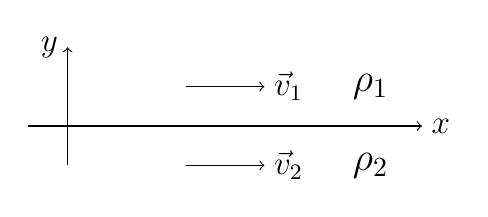
\begin{tikzpicture}
        \draw 
            [->, black] (-2,0)--(3,0) node[anchor=west]{\large $x$};
        \draw 
            [->, black] (-1.5, -0.5)--(-1.5, 1) node[anchor=east]{\large $y$};
        \draw 
            [->, black] (0,0.5)--(1,0.5) node[anchor=west]{\large $\vec{v}_{1}$};
        \draw 
            (2,0.5) node[anchor=west]{\Large $\rho_{1}$};
        \draw 
            [->, black] (0,-0.5)--(1,-0.5) node[anchor=west]{\large $\vec{v}_{2}$};
        \draw 
            (2,-0.5) node[anchor=west]{\Large $\rho_{2}$};
    \end{tikzpicture}
    \caption{Stratified fluids may give raise to instabilities.}
    \label{fig:stratified_fluid}
\end{figure}
Given these assumptions, the velocity fields may be written in terms of a scalar potential
\begin{equation*}
    \vec{v}_{i} = -\nabla\,\phi_{i}
\end{equation*}
Plugging this definition in Euler's equation yields (for example for fluid 1)
\begin{equation*}
    -\nabla(\partial_{t}\phi_{1}) +\nabla\left(\frac{v^{2}}{2}\right) = -\frac{\nabla \,p}{\rho}
\end{equation*}
Let's assume that the scalar potentials are composed of a constant term (temporally speaking) and a small space and time dependent fluctuation
\begin{equation*}
    \phi_{i} = -v_{i}x +\delta\phi_{i}
\end{equation*}
The condition for the fluid to be incompressible then becomes 
\begin{equation*}
    \nabla^{2}\delta\phi_{i} = 0
\end{equation*}
Say that the boundary between the two fluids can be parametrized by $y = \xi(x,t)$, then in the Lagrangian frame we have that 
\begin{equation*}
    \frac{\text{D}\xi}{\text{D}t} = \partial_{y}\delta\phi_{1} = -\partial_{y}\delta\phi_{2}
\end{equation*}
If we assume the pressure to be continuous at the interface and $\delta\phi_{i}$ to be plane waves of the form 
\begin{equation*}
    \delta\phi_{i} = B_{i}\exp(i(kx-\omega t)+k_{y})
\end{equation*}
we're able to find a dispersion relation for the system 
\begin{equation}
    \frac{\omega}{k} = \frac{\rho_{1}v_{1}+\rho_{2}v_{2}}{\rho_{1}+\rho_{2}} \pm \left[-\frac{\rho_{1}\rho_{2}(v_{1}-v_{2})^{2}}{(\rho_{1}+\rho_{2})}\right]^{1/2}
    \label{eq:KHi}
\end{equation}
Unless $v_{1} = v_{2}$, the argument of the square root is always negative, so the oscillation frequency has a purely imaginary component. When you plug that into the plane wave solution, you get an exponentially increasing amplitude for the wave, meaning that the system is unstable.
\par This is called \emph{Kelvin-Helmoltz instability}. The KH instability has characteristic vortices arising, which normally are damped at some point by viscosity, stopping the endless formation of vortices.
\par If we introduce a gravitational field in the vertical direction, we introduce a stabilizing factor in eq.\ref{eq:KHi}
\begin{equation}
    \frac{\omega}{k} = \frac{\rho_{1}v_{1}+\rho_{2}v_{2}}{\rho_{1}+\rho_{2}} \pm \left[\frac{g}{k}\frac{\rho_{2}-\rho_{1}}{\rho_{1}+\rho_{2}}-\frac{\rho_{1}\rho_{2}(v_{1}-v_{2})^{2}}{(\rho_{1}+\rho_{2})}\right]^{1/2}
    \label{eq:KH_RTi}
\end{equation}
Please note that even if $v_{1}=v_{2}$, the system may still be unstable. In fact, in such a scenario, the system is stable only if $\rho_{1}<\rho_{2}$ (referring to Fig.\ref{fig:stratified_fluid}), which actually makes sense: The less dense fluid must float over the denser fluid.
\par Conversely, the fluid is unstable if $\rho_{1}>\rho_{2}$ (\emph{Rayleigh-Taylor instability}). The RT instability presents characteristic "fingers" (or jets) extending from the less dense layer to the denser one.
\section{Properties of Turbulence}
To try giving a description of turbulence, we'll often perform a Reynolds' decomposition
\begin{equation*}
    \vec{v} = \langle\vec{v}\rangle +\delta\vec{v}
\end{equation*}
This allows us to write down an "averaged" version of the Navier-Stokes equation (\ref{eq:incompressible_ns}), in which a new term is coming out 
\begin{equation*}
    \partial_{t}\langle v_{i}\rangle+(\langle v_{j}\rangle\cdot\partial_{j})\langle v_{i}\rangle = -\frac{\langle \partial_{i}p\rangle}{\rho}-\partial_{i}\phi+\nu\partial^{2}_{j}\langle v_{i} \rangle+\nu\langle\delta v_{i}\delta v_{j} \rangle
\end{equation*}
The last term $\langle\delta v_{i}\delta v_{j} \rangle$ representing correlations between velocity fluctuations is notably absent in laminar flows. It adds a third source of stress to the stress tensor. If we assume the fluid to be incompressible, then eq.\ref{eq:stresstensor} becomes
\begin{equation*}
    \sigma_{ij} = -\langle p \rangle\delta_{ij}+\mu\left(\left[\partial_{j}\langle v_{i}\rangle +\partial_{i}\langle v_{j}\rangle \right]-\rho\langle\delta v_{i}\delta v_{j}\rangle\right)
\end{equation*}
The term containing the pressure is the \emph{isotropic stress}, the term containing the gradients of $v$ is the \emph{viscous stress} while the third new term is the \emph{Reynolds stress}, caused by fluctuations.
\par Making use of Wiener-Chinčin's theorem, we can link velocity fluctuations to fluctuations in kinetic energy. Usually the Reynolds' stress term is unpacked in a symmetric and an antisymmetric part defining the \emph{turbulent kinetic energy tensor}
\begin{equation*}
    \kappa(\vec{x},t) = \frac{1}{2}\langle \delta v_{i}\delta v_{i} \rangle
\end{equation*}
representing the mean kinetic energy (per unit mass) in the fluctuating velocity field. The \emph{deviatoric anisotropic part} is 
\begin{equation*}
    a_{ij} = \langle\delta v_{i}\delta v_{j}\rangle-\frac{2}{3}\kappa\delta_{ij}
\end{equation*}
which is the only component effectively transporting momentum. For a more detailed discussion about turbulence, you can check out the Fluid Dynamics course or give a look to \cite{Pope_2000}.
\subsection{Self-Similarity}
Suppose to have a quantity dependent on two independent variables $Q(x,y)$. Characteristic scales $Q_{0}(x)$ and $\delta(x)$ are defined for $Q,\,y$ respectively. Then the scaled variables are just 
\begin{equation*}
    \xi = \frac{y}{\delta(x)} \quad \tilde{Q}(\xi, x)=\frac{Q(x,\xi)}{Q_{0}(x)}
\end{equation*}
If the scaled dependent varibale is independent of $x$, i.e.
\begin{equation*}
    \exists\hat{Q}(\xi): \tilde{Q}(\xi, x) = \hat{Q}(\xi)
\end{equation*}
then $Q(x,y)$ is self-similar.
\par Self-similar fluids have really interesting properties that more often than not are able to greatly simplify what we're working with. Since understanding what a self-similar solution actually is is often more complicated than using it, we'll give two examples.
\par The first we've already seen: It's eq.\ref{eq:lane_emden}. If you recall, we've defined \emph{scales} for both the density and the radial distance and proceeded to tranform our messy second order ODE in a still messy but at least adimensional second order ODE.
\par Doing this has the perk that once you've found a solution for $\phi(\eta)$, you already have a solution for whatever density and/or radial distance scale may come to your mind.
\par Another example, you can find in the Schwartzschild metric for non-rotating, spherically symmetric black holes. General relativity and Birkhoff's theorem grants us that 
\begin{equation}
    \text{d}s^{2} = -\left(1-\frac{R_{s}}{r}\right)\text{d}t^{2}+\left(1-\frac{R_{s}}{r}\right)^{-1}\text{d}r^{2}+r^{2}\text{d}\Omega_{(2)}^{2}
    \label{eq:Schwartzschild_metric}
\end{equation}
is the only possible spherically symmetric solution to the Einstein's equation in vacuum\,\footnote{Please note that we're using Carroll's \cite{carroll} convention for the signature of the metric, which, incidentally, isn't the same used in the GR course.} (well, assuming there actually \emph{is} something somewhere in space-time inducing this metric).
\par From (\ref{eq:Schwartzschild_metric}) is perhaps even simpler understanding what a self-simlar solution is: Just plug $y = R_{s}/r$ and you'll find that the metric is completely specified up to a factor of $R_{s}$, which contains all the details of the source of the curvature.
\subsection{Kolmogorov's scales}
In a revolutionary article of 1941, the Russian physicist A. V. Kolmogorov developed one of the most incredible theories about the structure of turbulence in incompressible fluids \cite{1991RSPSA.434....9K}.
\par we shall start assuming we're in presence of a fully turbulent flow with $Re = UL/\nu \gg 1$ and Richardson's theory about the "energy cascade" to hold: That means turbulence can be considered to be composed of eddies of different sizes which can be described through the tern of parameters $l,\,u(l),\,\tau(l)=l/u(l)$.
\par The eddies of the largest scales are characterized by lengthscale $l_{0}$ comparable to $L$ (the dimension of the system housing the turbulent liquid) and have characteristic velocity $u(l_{0}) \approx (2\kappa/3)^{1/2}\approx U$.
\par Larger eddies are unstable. Pretty much like boybands in the prime of their careers, they end up breaking apart, transferring energt to "smaller" eddies. This \emph{energt cascade} continues until the Reynolds' number $Re(l)$ is sufficiently small that the eddy motion is stable.
\par The energy dissipation rate $\varepsilon$ is determined by the transfer of energy from the largest eddies and is \textbf{independent of the kinematic viscosity $\nu$}.
\par Here comes to play Kolmogorov's key hypothesis. Ar sufficiently high $Re$, the small-scale turbulent motions are claimed to be \emph{isotropic}. Let's call $l_{I}$ the lengthscale demarcation between anisotropic large and isotropic small eddies.
\par Isotropy in this case means that all directional information is lost, as well as all information about the geometry of larger eddies. In a sense then, the statistics of small-scale motions are in a sense \emph{universal}.
\subsubsection*{1st hypothesis of self-similarity}
In every turbulent flow with $Re\gg 1$, the statistics of the small-scale range have a universal form determined by $\varepsilon,\,\nu$ alone. We can define \emph{Kolmogorov's scale} so that $Re=1$
\begin{align*}
    l_{\eta} &= \left(\frac{\nu^{3}}{\varepsilon}\right)^{1/4}\\
    u_{\eta} &= (\varepsilon\nu)^{1/4}\\
    \tau_{\eta} &= \left(\frac{\nu}{\varepsilon}\right)^{1/2}
\end{align*}
characterizing the smallest dissipative eddies.
\par The implications are astounding. Consider a point $\vec{x}_{0}$ at a time $t_{0}$ for a fully-developed turbulent flow. In terms of Kolmogorov's scales, we can define adimensional coordinates and velocities
\begin{align*}
    \vec{y} &= \frac{\vec{x}-\vec{x}_{0}}{\eta} \\
    \omega(\vec{y}) &= \frac{\vec{U}(\vec{x},t_{0})-\vec{U}(\vec{x}_{0},t_{0})}{u_{\eta}}
\end{align*}
Since it is not possible to form a non-dimensional quantity with $\varepsilon,\,\nu$, the universal form of the statistics of the non-dimensional field $\omega(\vec{y})$ \textbf{cannot depend on $\varepsilon,\,\nu$}. That means that on not-too-large scales, $\omega(\vec{y})$ is statistically isotropic and identical at all points.
\par That implies that all fully-developed turbulent flows have velocity fields statistically similar.
\subsubsection*{2nd hypothesis of self-similarity}
In every turbulent flow with $Re \gg 1$, the statistics of motion of scale $l$ in the range $l_{0}\gg l \gg \eta $ have a universal form determined by $\varepsilon$ alone, independent of $\nu$
\input{chapters/kolmogorov}
which means the effect of viscosity is relevant only when we're dealing with lengthscales smaller than $\eta$. It seems like a honest assumption: a Reynolds' number smaller than 1 (\ref{eq:reynoldsnumber}) requires viscous forces to be greater than the inertial driving. By construction, Kolmogorov's scales identify the conditions for which $Re = 1$, so all is consistent.
\par We're not going to show explicitly, but from the two hypothesis of self-similarity we can conclude something really important. In the equilibrium range ($l<l_{EI}$, see Fig.\ref{fig:kolmogorov_scales}) the spectrum is a universal function of $\varepsilon,\,\nu$. But then, the second hypothesis of self-similarity tells us that in the inertial subrange statistics cannot depend on $\nu$. 
\par If we were to calculate explicitly velocity correlations to plug them into the Wiener-Chinčin's theorem, we'd get an expression for how energy is distributed into modes $\kappa$ (the wavenumber)
\begin{equation}
    E(\kappa) = C \varepsilon^{2/3}\kappa^{-5/3}
    \label{eq:energy_modes}
\end{equation}
Here $C$ is a universal constant. What's most fascinating about (\ref{eq:energy_modes}) is that not only it has been tested to be actually true for many types of different fluids, but it is also valid if we relax the condition of incompressibility\footnote{The $\kappa$ dependence is unchanged, but a dependence on the \emph{Mach number} $M$ is introduced.}.
\par The typical velocity fluctuation in a fluid can be evaluated from the root mean square 
\begin{equation*}
    \delta \bar{v} = \sqrt{\langle\delta v^{2}\rangle} > 0
\end{equation*}
introducing a non-thermal broadening in the spectrum lines (see "Line Broadening" in Chapter \ref{ch:2}). In principle, we have only access to velocity-fluctuations on the line of sight (since that's what we can directly measure in observations), hence the difficulty of recognizing the occuring of turbulence in most objects of astrophysical interest. And that is most frustrating since, for example, the ISM\footnote{i.e. \emph{InterStellar Medium}.} has a Reynolds' number of roughly $10^{8}$.
\par To actually resolve the spatial structure of turbulence we require a resolution of astrophysical proportions (pun intended), at least proportional to $Re^{-1}$.
\par As a concluding note, in the presence of magnetic fields, eq.\ref{eq:energy_modes} is modified $E_{M} \propto \kappa^{-2}$. In principle, both dependencies can be present at once, allowing us to differentiate between neutral and magnetized phases.
\section{Sound waves and shocks}
At this point, it should come to no surprise to you that we're coming back once more to our initial, easy rising-bubble model to further complicate it. We've already seen that as a consequence of its vertical motion, instabilities arise (\ref{eq:KH_RTi}), tranforming our cool little bubble in a swirly mess. 
\par Another fairly important consequence of the bubble's motion is the arising of pressure differences between the material itself and the wake\footnote{\emph{N.d.T.}: in Italian, it should sound something like "scia".} coming after the bubble.
\par For this section (and many more in the Gravitation Part) I'll be following \cite{Frank_King_Raine_2002}. Relevant paragraphs for this section are §2.4 and §3.8.
\par Let's write Euler's equation and the continuity equation (\ref{eq:lagrangianframe}) in a conservative form 
\begin{align*}
    \partial_{t}(\rho\vec{v}) + (\vec{v}\cdot\nabla)(\rho\vec{v}) &= -\nabla\, p\\
    \partial_{t}\rho +\nabla(\rho\vec{v}) &= 0
\end{align*}
and look for perturbations around the equilibrium solution.
\begin{align*}
    \vec{v} &= \vec{v}_{0} + \vec{v}_{1}\\
    p &= p_{0}+p_{1}\\
    \rho &= \rho_{0}+\rho_{1}
\end{align*}
Since Euler's equation (and by extension, Navier-Stokes' equation) is invariant under Galileian transformations, we can set $\vec{v}_{0} = 0$. We shall also assume a one dimensional motion and a barotropic equation of state, allowing us to linearize our equations.
\par Quantities with the "0" subscript are assumed to be uniform and stationary. Keeping only first order quantities, we find
\begin{align*}
    \partial_{t}\rho_{1}+\rho_{0}\partial_{x}v_{1} &= 0\\
    \rho_{0}\partial_{t}v_{1} +\left(\frac{\partial p}{\partial \rho}\right)_{0}\frac{\partial\rho_{1}}{\partial x} &=0
\end{align*}
Cross derivating the two equations and plugging in one equation into the other, we end up with 
\begin{equation}
    \partial^{2}_{t}\rho_{1}-\left(\frac{\partial p}{\partial \rho}\right)_{0}\partial^{2}_{x}\rho_{1} = 0
    \label{eq:soundwaves}
\end{equation}
which is a hyperbolic equation describing propagating density waves!
\par We can identify
\begin{equation*}
    c_{s}^{2} = \left(\frac{\partial p}{\partial \rho}\right)_{0}
\end{equation*}
as the \emph{speed of sound} in the fluid. Sometimes $c_{s}$ is also said to be the compressibility of the fluid.
\par Since $c_{s}$ is the speed at which pressure (or density) perturbations travel through the gas, it limits the rapidity with which the fluid can react to such changes. For example, if the pressure in one part of a region of the fluid of characteristic size $L$ is suddenly changed, the other parts of the region cannot respond to this change until a time of order $L/c_{s}$, the sound crossing time, has elapsed.
\par In a sense, $c_{s}$ is also the velocity at which causality travels in the fluid. Thus, if we were to consider a \emph{supersonic flow}, then the fluid cannot respond on the flow time $L/\left|\vec{v}\right|$, so pressure gradients have little effect on the flow. At the other extreme, for subsonic flow the fluid can adjust in less than the flow time, so to a first approximation the fluid behaves as if in hydrostatic equilibrium.
\par The density dependence of the sound speed implies that regions of higher than average density have higher than average sound speeds, a fact which gives rise to the possibility of \emph{shock waves}.
\begin{figure}[h!]
    \centering 
    \includegraphics[width=0.7\textwidth]{img/shockformation}
    \caption{The formation of a shock wave. Credits: Frank, King and Raine.}
    \label{fig:shock_dev}
\end{figure}
\par In a shock relevant fluid quantities change on lengthscales of the order of the mean free path and this is represented as a discontinuity in the fluid.
\subsection{Rankine-Hugoniot junction conditions}
\par Since discontinuities are introduced into the picture, we can no longer use differential quantities to describe conservations. The solution to this problem is easily found looking into \emph{integral quantities}.
